\documentclass[12pt, letterpaper]{article}

\usepackage[utf8]{inputenc}
\usepackage[margin=1in]{geometry}
\usepackage{comment}
\usepackage{caption}%for table captions

\usepackage[shortlabels]{enumitem}%for (a) (b) (c) enumerate use [(a)] like so:
%\begin{enumerate}[(a)]
\usepackage{bm}%bold symbols in math mode
\usepackage{amsmath}%allows text in math mode e.g. \text{}
\usepackage{amssymb}%allows \checkmark
\usepackage{physics}%allows use of \abs{}. Absolute value.

\usepackage{listings}%Typeset Python
%Here is an example of how to do that
%\begin{lstlisting}[language=Python, basicstyle=\tiny]
%#Here is some test Python
%def yay():
%    print("hi")
%\end{lstlisting}

\usepackage{graphicx}%for images
%\includegraphics{uploaded-file-name}

\usepackage{float}%supposedly will allow the use of [H] for table and figure positioning

\title{COSC 5010-03 Practical Machine Learning Fall 2023 Pipeline Optimization Report}
\author{Michael Elgin}
\date{November 22, 2023}

\begin{document}

\maketitle

\section{Introduction} %What problem are you solving, how are you going to solve it.

Parts of a machine learning pipeline include not only the choice of model (algorithm) and the task of tuning the associated hyperparameters, but various choices about how to preprocess the data. This report explores the effect of normalization, feature reduction, and sample reduction (outlier removal) on the wine quality dataset\footnote{https://archive.ics.uci.edu/dataset/186/wine+quality}. The effect of these preprocessing changes is examined on a linear regression model for regression, and a decision tree and random forest for classification.

\section{Dataset Description} %Describe the data you're using, e.g. how many features and observations, what are you predicting, any missing values, etc.

The wine quality dataset is standard tabular data. There are 2 datasets for each color of red and white. Both contain 11 features, all of which are continuous. The target is a discrete value which is the assigned quality of the wine. For the regression tasks, the white wine dataset is used to evaluate models. For classification tasks, both datasets are concatenated, with the target being changed to be the color of the wine, with 0 being assigned to red and 1 to white.

\section{Experimental Setup} %What specifically are you doing to solve the problem, i.e. what programming languages and libraries, how are you processing the data, what machine learning algorithms are you considering, how are you evaluating them, etc.

All computation is done with the Python programming language. Scikit-learn is used to construct models. Pandas is used to load and preprocess the data.

For regression, performance is the mean absolute percentage error. This is defined by taking the difference between the predicted value of the model and the actual value, then dividing by the actual value. Then the mean of all of those is taken. More formally:

$$
    GE_{Regression\ model}(\hat{f}, \bm{X}_{test}, \bm{y}_{test}) = \frac{100}{|\bm{X}_{test}|} \sum_{i=1}^{|\bm{X}_{test}|} \abs{\frac{\hat{f}(\bm{X}_{test,i}) - \bm{y}_{test,i}}{\bm{y}_{test,i}}}
$$

For classification, the performance metric is standard accuracy:

$$
    GE_{Classification\ model}(\hat{f}, \bm{X}_{test}, \bm{y}_{test}) = \frac{\sum_{i=1}^{|\bm{X}_{test}|}l_{0,1}(\hat{f}(\bm{X}_{test,i}), \bm{y}_{test,i})}{|\bm{X}_{test}|}
$$

$$
Acc_{Classification\ model} = (1 - GE_{Classification\ model}) * 100
$$

For the linear model, no hyperparameters are tuned. For the tree and forest, Bayesian optimization is used for trying hyperparameter configurations. This tunes the max depth and minimum samples for a split in the models. The minimum max depth is 1 and minimum minimum samples for a split is 2. Their maxes are 64 and 16,384 respectively. The forest contains 100 trees.

$$
\text{max depth} = 2^x, x \in [0,6]
$$

$$
\text{min samples} = 2^x, x \in [1,14]
$$

The process uses nested resampling. The outer loop (for the unbiased performance estimate) uses 2 folds, the inner loop (for the search itself) uses 2 folds.

The first pipeline optimization option is whether or not to normalize the data. This consists of z-scoring the data according to the formula

$$
z = \frac{(X - \mu)}{\sigma}
$$

Regression will normalize the target (quality) as well, but classification will not do this to color.

The second pipeline optimization option is to reduce the amount of features in the data. This step will remove all features except for the top features that are most strongly positively or negatively correlated with the target.

The third pipeline optimization option is to reduce the amount of samples in the data by removing outliers. Outliers are determined by whether or not they are outside of the range

$$
[Q1 - 1.5 \cdot IQR, Q3 + 1.5 \cdot IQR]
$$

Where Q1 is the first quartile, Q3 is the third quartile, and IQR is the interquartile range. For a sample, if any value in any of the feature columns is out of range, the sample will be removed. The target is not a column considered.

For both regression and classification, the settings for the pipeline are optimized together (not independently) along with the hyperparameters as applicable.

\section{Results} %Description of what you observed, including plots.

pipe.ipynb prints every combination of pipeline settings with MAPE/accuracy.

\subsection{Regression}

The most interesting trends are plotted in figure \ref{reg_plt}.

\begin{figure}[H]
    \centering
    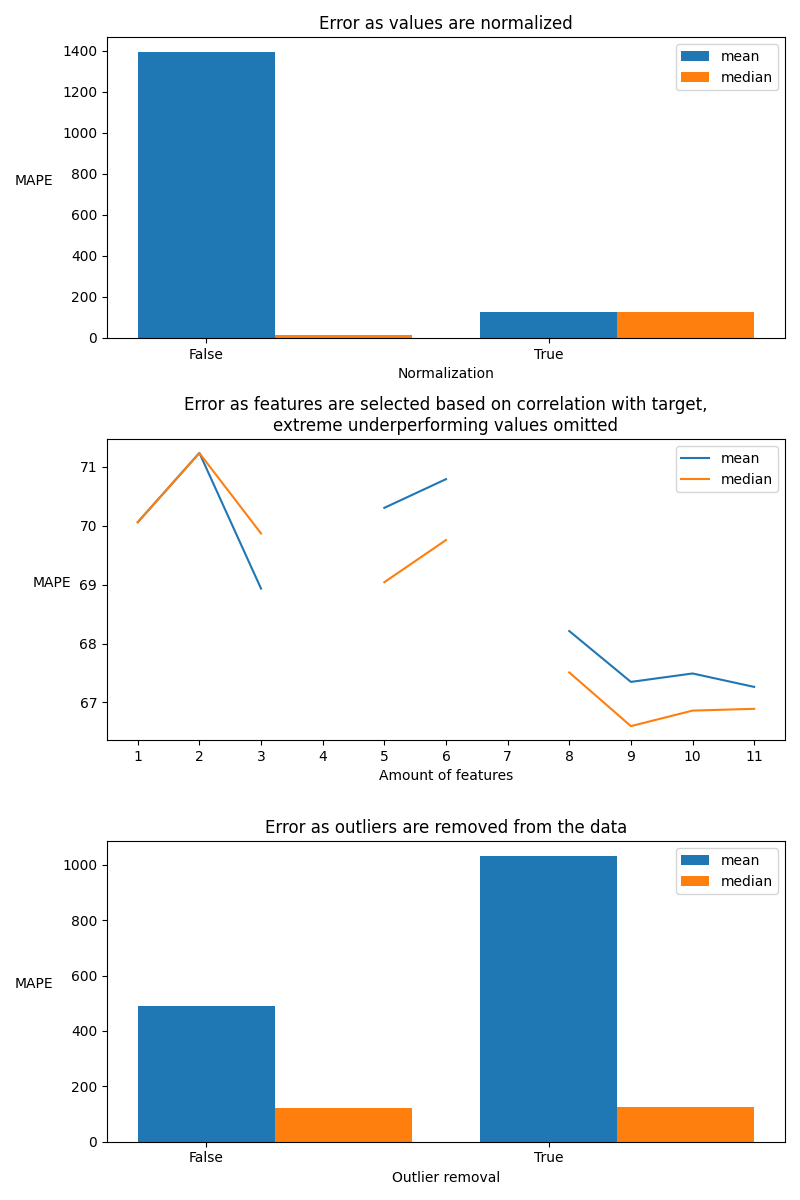
\includegraphics[scale=0.7]{regression_performance.png}
    \caption{Regression performance trends}
    \label{reg_plt} % For referencing the figure later in the document
\end{figure}

The individual best case was to not normalize the data, not reduce the samples, but reduce the features from 11 down to 9. Furthermore, a facet of the optimization process worth highlighting is that not normalizing the data occasionally causes extreme outliers in the MAPE, i.e. it mostly produces much better MAPE values but occasionally an extremely large MAPE that enlarges the average, which was reflected in the stark difference between mean and median MAPE values there.

\begin{comment} old table before expanding feature reduction to every amt
\begin{table}[H]
\centering
\caption{Regression model pipeline optimization effects}
\label{reg_table}
\begin{tabular}{c|c|c|c} % l for left-aligned column, c for centered columns
Normalize   & Feature Reduction & Sample Reduction & MAPE \\ \hline
            &                   &                  & 11.566 \\
            &                   & \checkmark       & 11.668 \\
            & \checkmark        &                  & 11.907 \\
            & \checkmark        & \checkmark       & 11.930 \\
\checkmark  &                   &                  & 122.117 \\
\checkmark  &                   & \checkmark       & 123.706 \\
\checkmark  & \checkmark        &                  & 126.153 \\
\checkmark  & \checkmark        & \checkmark       & 131.229 \\            
\end{tabular}
\end{table}

From table \ref{reg_table} it can be seen that all pipeline options made performance worse. In the case of feature reduction and sample reduction, trivially so. In the case of Normalization, performance was made drastically worse.
\end{comment}

\subsection{Classification}

The optimal pipeline was with the forest, with the values in table \ref{best_forest_table}.

\begin{table}[H]
\centering
\caption{Best pipeline values overall}
\label{best_forest_table}
\scalebox{0.9}{
\begin{tabular}{c|c|c|c|c|c} % l for left-aligned column, c for centered columns
Normalize   & Feature Amount & Sample Reduction & Max Depth & Min Samples Split & Acc \\ \hline
   False    &    10           &    True         & 64        &  662              &  0.995\\
\end{tabular}}
\end{table}

Table \ref{best_tree_table} shows the best pipeline values obtained for the tree.

\begin{table}[H]
\centering
\caption{Best pipeline values for the tree}
\label{best_tree_table}
\scalebox{0.9}{
\begin{tabular}{c|c|c|c|c|c} % l for left-aligned column, c for centered columns
Normalize   & Feature Amount & Sample Reduction & Max Depth & Min Samples Split & Acc \\ \hline
   True    &    7           &    True         & 34        &  950              &  0.986\\
\end{tabular}}
\end{table}

Next, the accuracy of the tree and forest are scattered together to see if they tend to both improve together or not.

\begin{figure}[H]
    \centering
    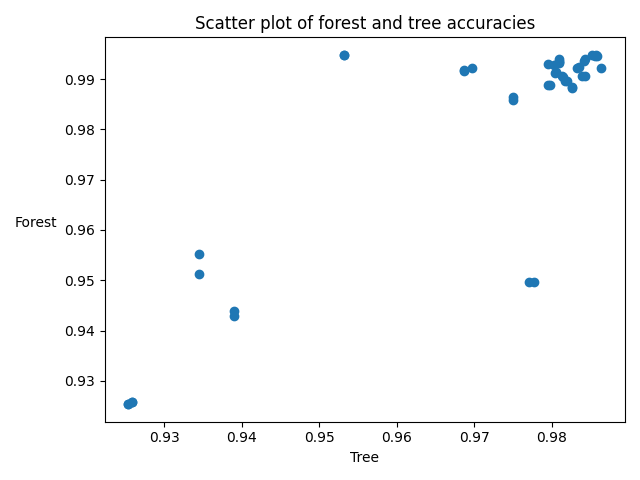
\includegraphics[scale=0.7]{accuracy_scatterplot.png}
    \caption{Accuracy scatterplot}
    \label{acc_plt} % For referencing the figure later in the document
\end{figure}

As is seen from figure \ref{acc_plt}, a change in the pipeline was generally either good for both models or bad for both models.

The trends of optimization are shown in figure \ref{cls_plt}.

\begin{figure}[H]
    \centering
    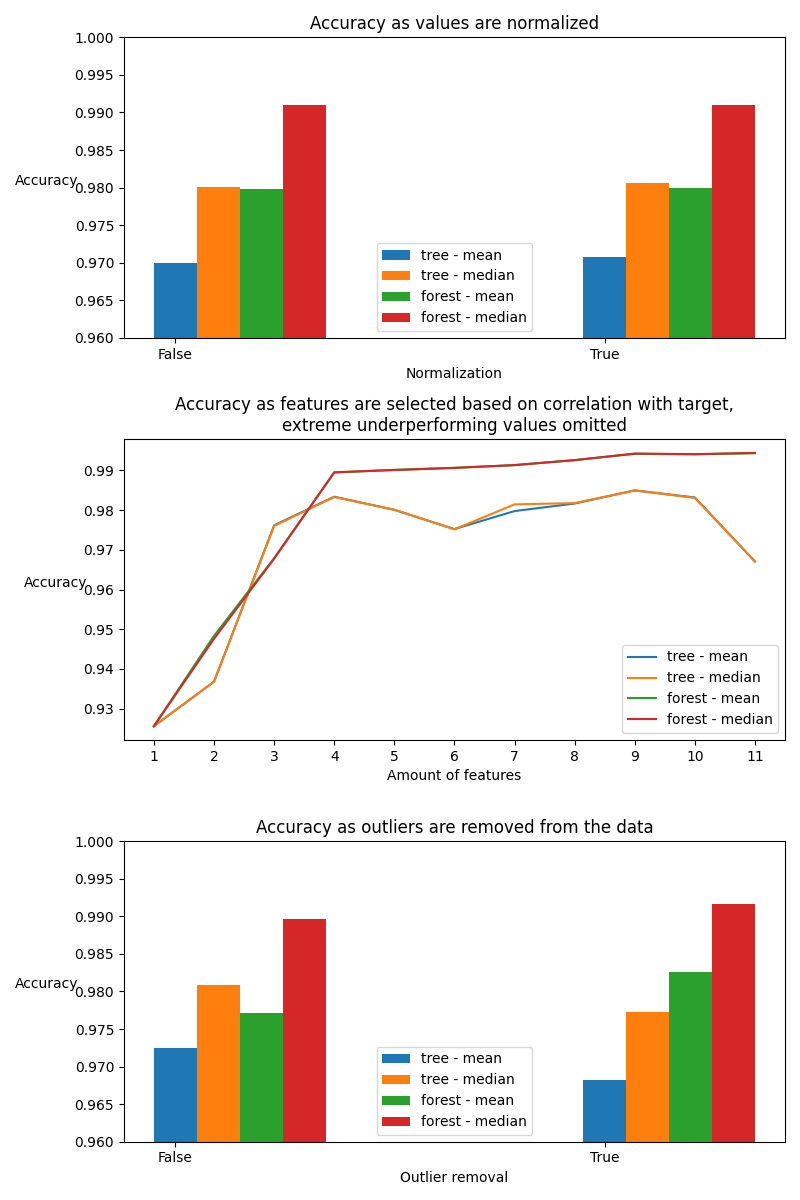
\includegraphics[scale=0.7]{classification_performance.png}
    \caption{Classification performance trends}
    \label{cls_plt} % For referencing the figure later in the document
\end{figure}

From the first plot, it is clear that normalization had very little affect on the tree and forest, which was a world of difference compared to what happened with linear regression. In the second plot, it is is clear that the forest benefitted from having all the features whereas the tree was slightly better off with removing a few of the features that were least correlated with the target. Third, the value of outlier removal was very model dependent, with the forest getting better but the tree getting worse.

The main takeaways from these results is that firstly pipeline tuning has the \emph{potential} to improve performance, but likewise is it very easy to cause harm with it. Second, when all parts are optimized together, there is a tendency for changes in the pipeline optimization to affect model hyperparameters as well. Third, the value of pipeline optimization steps are, in principle, heavily dependent on whether the situation is a regression or classification as well as the model class itself.

\begin{comment} old table before expanding feature reduction to every amt
\begin{table}[H]
\centering
\caption{Classification model pipeline optimization effects}
\label{cls_table}
\begin{tabular}{c|c|c|c|c|c} % l for left-aligned column, c for centered columns
Normalize   & Feature Reduction & Sample Reduction & Max Depth & Min Samples Split & Acc \\ \hline
            &                   &                  & 32     &  2    &  0.984 \\
            &                   & \checkmark       & 8     &   2    &  0.987 \\
            & \checkmark        &                  & 8     &   4    &  0.980\\
            & \checkmark        & \checkmark       & 4     &   2    &  0.983 \\
\checkmark  &                   &                  & 32     &   2    &  0.984\\
\checkmark  &                   & \checkmark       & 8     &   2    &  0.988 \\
\checkmark  & \checkmark        &                  & 8     &   4    &  0.980\\
\checkmark  & \checkmark        & \checkmark       & 4     &   2    &  0.983\\            
\end{tabular}
\end{table}

In the case of classification, pipeline options had merit. Sample reduction allowed for better performance from the decision tree. Feature reduction was harmful. Normalization had little to no effect.

The main takeaways from these results is that firstly pipeline tuning has the \emph{potential} to improve performance, but likewise is it very easy to cause harm with it. Second, when all parts are optimized together, there is a tendency for changes in the pipeline optimization to affect model hyperparameters as well. For example, when features and samples were reduced in the data for the decision tree, the tree was better off with the more strict depth limits of 8 and 4, but with the full features and samples 8 or 4 would likely be too restrictive, hence the max depth of 32. Third, the value of pipeline optimization is, in principle, heavily dependent on whether the situation is a regression or classification as well as the model class itself.
\end{comment}

\section{Code} %Add the code you've used as a separate file.

The associated code is in pipe.ipynb

\end{document}